\documentclass[11pt,a4paper]{article}

\usepackage[margin=2.4cm]{geometry}
\usepackage{amsmath,amssymb}
\usepackage{graphicx}
\usepackage{booktabs}
\usepackage[round,authoryear]{natbib}
\usepackage[dvipsnames]{xcolor}
\usepackage[colorlinks=true,linkcolor=RoyalBlue,citecolor=RoyalBlue,
            urlcolor=RoyalBlue]{hyperref}
\usepackage{microtype}

\newcommand{\cvec}{\mathbf{c}}
\newcommand{\Sq}{\Sigma_{Q}}
\newcommand{\Sb}{\Sigma_{B}}
\newcommand{\dd}{\mathrm{d}}
\newcommand{\Hsame}{H_{\rm same}}
\newcommand{\Hfield}{H_{\rm field}}
\newcommand{\Hbkg}{H_{\rm bkg}}
\newcommand{\kms}{\,\mathrm{km\,s^{-1}}}

\title{Colour evidence that the companion of a quasar is\\
       itself a quasar at the same redshift}
\author{Method note for \texttt{qso\_pcolor}}
\date{\today}

\begin{document}
\maketitle

\begin{abstract}
\noindent
A quasar has a spectroscopic redshift $z_0$; a companion a few arcseconds away
has broadband photometry and nothing else. We want to know how strongly the
companion's colours support the hypothesis that it is a quasar at $z\simeq z_0$.
This note sets out the method implemented in \texttt{qso\_pcolor}: a
class-conditional colour--redshift density for quasars, a local
colour--magnitude--sky density for the field population, explicit surface
densities that convert those into intensities, and a three-hypothesis posterior
that includes quasars at the \emph{wrong} redshift as a competing explanation.
We show that the redshift-match window enters the answer as a pure
multiplicative constant, derive the window-free statistic $R$ that follows from
that, and explain why $R$ rather than a posterior probability is the quantity to
rank on. All figures are built from DESI DR1 spectroscopy and Legacy Surveys
DR9 imaging. Applied to those data, the statistic separates quasars from the
field population by about fourteen natural logarithms but separates
same-redshift from wrong-redshift quasars by only about two: these bands
identify quasars well and place them in redshift only weakly, which is the
central practical constraint on the method.
\end{abstract}

\section*{The method in plain words}
\addcontentsline{toc}{section}{The method in plain words}

An orientation before the formalism. Everything asserted here is developed, and
qualified, in the sections that follow.

\paragraph{The question, and what is in scope.} We have a quasar whose redshift
has been measured from a spectrum, and a neighbour a few arcseconds away for
which we have only photometry --- a brightness in each of a handful of filters.
We want to know whether that neighbour is also a quasar, at the same redshift.
The pipeline scores only companions far enough from the primary that the survey
photometry treats them as separate sources; closer pairs need image-level work
that is not attempted here (\S\ref{sec:limitations}).

\paragraph{How we learn what quasars look like.} We take the quasars DESI has
observed spectroscopically --- about $80{,}000$ in the patch used for the
figures --- and attach the brightnesses that the Legacy Surveys imaging measured
for those same objects. The two catalogues share an identifier, so the
photometry is attached by name rather than by position; removing objects that
appear twice under different identifiers is a separate step
(\S\ref{sec:validation}). That gives a cloud of points in colour space with a
measured redshift attached to each. We fit a separate distribution in each of a
set of \emph{overlapping} redshift slices, and blend the two neighbouring
distributions according to where in between a given redshift falls. The result
answers: \emph{if this object is a quasar at redshift $z$, how likely are these
colours?}

One property of that sample must be carried forward: DESI selects quasars for
spectroscopy using a classifier built on these very colours. What we learn is
therefore the colour distribution of quasars \emph{that DESI would target}, not
of quasars in general.

\paragraph{Why measurement error is handled explicitly.} Every measured colour
carries an uncertainty, and those uncertainties are correlated between colours
because the colours share bands. Fitting the observed cloud would give a locus
broader than the true one, and would make unusual colours look less unusual than
they are. So we fit the \emph{underlying} distribution, using each training
object's full measurement covariance, and then --- when scoring a candidate ---
add that candidate's own covariance back in. A noisy candidate is thus compared
against an appropriately blurred locus, not against an artificially sharp one.

\paragraph{What we use for the competing population.} Not stars alone. We take
every source in the same imaging that passes the same quality cuts as the
candidate, and model its colours the same way: stars, faint galaxies, blends,
whatever the survey actually contains. The reason is that a chance neighbour is
drawn from everything that is there. Estimating that population directly from
catalogue detections avoids having to reconstruct what lies below the detection
limit, though it still requires that the candidate cuts and the usable sky area
match. Because this population changes across the sky and with depth, we fit it
separately in patches of sky and in bins of brightness, falling back to coarser
patches where a cell holds too few objects.

One honest complication: this sample is not currently purged of quasars, so the
``quasar'' and ``everything else'' categories overlap and part of the quasar
population is counted twice. Their fraction among all sources is tiny, but that
does not bound the effect where quasar colours live, which is the only place it
matters. The size of it has not yet been measured (\S\ref{sec:background}).

\paragraph{How the two are compared.} Two colour distributions alone cannot
answer the question. They give the relative colour evidence --- useful, and
reported --- but not a probability, because that also depends on how many
objects of each kind exist at this brightness on this part of the sky. So each
distribution is multiplied by a surface density: quasars per square degree per
unit brightness \emph{per unit redshift}, and field sources per square degree per
unit brightness. The quasar quantity is then summed over redshift, separately
inside and outside the declared match window, which is what makes the two
comparable. What come out are expected-count densities for three possibilities:

\begin{itemize}
\item a quasar at the primary's redshift,
\item a quasar at some \emph{other} redshift,
\item anything else in the imaging.
\end{itemize}

The middle one is not a refinement. A genuine quasar behind the primary at a
quite different distance looks nothing like a star, so a two-way
quasar-versus-star comparison would count it as evidence for a companion. For a
pair search that is the main way of being wrong.

\paragraph{Why the answer is a ranking rather than a verdict.} Colours locate a
quasar in redshift only loosely: on our models the redshift posterior has a
median standard deviation of about $0.6$, and is often multimodal. A physically
motivated pair window of $\pm2000\kms$ spans about $0.037$ in redshift at
$z=1.8$. The window is far narrower than the measurement, so only a small part
of a candidate's redshift probability can ever fall inside it, and the resulting
probability is correspondingly small. Strong colour evidence can therefore
coexist with a small probability of falling inside such a narrow window; a small
number is not by itself a verdict against the candidate.

For that reason we report a statistic that the width of the window barely
affects --- exactly so in the limit of a narrow window, approximately so in
practice --- and convert it to a probability only at the end, for a window the
user declares. Candidates are ordered by that statistic; spectroscopy decides.
Note also that even a confident answer here is a statement about colours and
populations, not about whether two quasars are physically bound: that needs a
clustering model this pipeline deliberately leaves out.

\paragraph{What the illustrative numbers do and do not show.} Applied to the
sky patch used for the figures, the ranking statistic puts quasars far from the
general field population, and same-redshift quasars only modestly above
wrong-redshift ones --- medians differing by about $14$ and about $2.3$ natural
logarithms respectively (\S\ref{sec:howmuch}). These are in-sample comparisons
from one untuned model at one redshift, with the hardest intermediate cases
absent, so they indicate the dynamic range available rather than any measured
purity or completeness. Read at that level, they say that these filters identify
quasars much better than they place them in redshift. Whether extra filters with
a steeper colour--redshift dependence would improve matters is a reasonable
expectation from \S\ref{sec:whatsets}, not something demonstrated here.

\clearpage

\section{The question, and the question that can be answered}
\label{sec:question}

The scientific target is physical quasar pairs. The observational situation is
that one member has a spectrum and the other does not, and obtaining the second
spectrum is expensive. A method that ranks companions by how quasar-like their
colours are \emph{at the primary's redshift} therefore decides where telescope
time goes.

Two things must be separated at the outset, because conflating them is the
standard failure of this kind of analysis.

\paragraph{A likelihood is not a probability.} The quantity
$p(\cvec\mid Q,z_0)$ --- how probable these colours are \emph{if} the object is
a quasar at $z_0$ --- says nothing on its own about whether the object is a
quasar. Turning it into a probability requires knowing how many quasars and how
many other objects exist at this brightness and sky position. We therefore
compute and report both, and never let the first be read as the second.

\paragraph{Two hypotheses are not enough.} A calculation that pits ``quasar at
$z_0$'' against ``star'' will assign a high probability to a genuine quasar at
$z=2.6$ sitting beside a primary at $z=1.4$, because such an object is indeed
nothing like a star. For a pair search that is not a detail; it is the dominant
contaminant. The competing hypotheses must include field quasars.

\section{Hypotheses and intensities}
\label{sec:hypotheses}

Let $\cvec$ be a vector of colour/shape features, $m$ a reference magnitude, and
$(\ell,b)$ Galactic coordinates. We consider

\begin{center}
\begin{tabular}{ll}
\toprule
$\Hsame$ & a quasar whose redshift matches $z_0$ under a declared window \\
$\Hfield$ & a quasar at any other redshift \\
$\Hbkg$ & anything else in the imaging catalogue at this $m$ and $(\ell,b)$ \\
\bottomrule
\end{tabular}
\end{center}

$\Hbkg$ is deliberately not ``star''. The population a chance projection draws
from is everything the imaging contains --- stars, compact galaxies,
unclassified blends --- and that population has the decisive practical
advantage of requiring no selection function, because it is exactly the set of
objects being counted (\S\ref{sec:background}).

We work with \emph{intensities}: expected counts per unit sky area, per unit
magnitude, per unit volume of colour space. Writing $W(z\mid z_0)\in[0,1]$ for
the redshift-match weight, $\Sq(z,m)$ for the quasar surface density and
$\Sb(m,\ell,b)$ for the background surface density,
%
\begin{align}
\lambda_{\rm same} &= \int W(z\mid z_0)\,\Sq(z,m)\,p(\cvec\mid Q,z)\,\dd z,
\label{eq:lam_same}\\
\lambda_{\rm field} &= \int \bigl[1-W(z\mid z_0)\bigr]\,\Sq(z,m)\,
                        p(\cvec\mid Q,z)\,\dd z,
\label{eq:lam_field}\\
\lambda_{\rm bkg} &= \Sb(m,\ell,b)\,p(\cvec\mid B,m,\ell,b).
\label{eq:lam_bkg}
\end{align}
%
All three carry the same units, so their ratios are meaningful, and
%
\begin{equation}
p_{\rm same} =
\frac{\lambda_{\rm same}}
     {\lambda_{\rm same}+\lambda_{\rm field}+\lambda_{\rm bkg}} .
\label{eq:posterior}
\end{equation}
%
Alongside this we always report the prior-independent colour Bayes factor
%
\begin{equation}
\log \mathrm{BF} = \log p(\cvec\mid Q,z_0) - \log p(\cvec\mid B,m,\ell,b),
\label{eq:bf}
\end{equation}
%
which depends on the two density models but on neither surface density. If the
surface densities change, \eqref{eq:posterior} must move and \eqref{eq:bf} must
not; this is enforced by a unit test rather than by intention.

\section{Photometric features and their covariance}
\label{sec:features}

\subsection{Relative fluxes}

The default feature vector divides each band's flux by a reference band,
$r_j = f_j/f_a$, giving a representation of spectral shape that is independent
of overall brightness. Fluxes, not magnitudes, are the natural variable: a faint
source can legitimately have a \emph{negative} measured flux, which is a real
measurement of a faint object and carries information about the spectral energy
distribution. Converting to a magnitude would discard it, and replacing it with
a limit or a clipped value would bias the locus. We therefore never clip, floor,
or drop a band because its flux came out negative or low in signal-to-noise. A
band is unusable only when the survey says so --- zero inverse variance, zero
exposures, or a mask bit --- and that is expressed through an observed-dimension
mask rather than by imputing a value.

The covariance follows by the Jacobian. With independent band fluxes of variance
$v_j$,
%
\begin{equation}
\bigl[\mathbf{C}_r\bigr]_{jk} =
\frac{\delta_{jk}\,v_j}{f_a^{2}} + \frac{r_j r_k\, v_a}{f_a^{2}},
\label{eq:cov_relflux}
\end{equation}
%
whose second term is a dense, strictly positive contribution from the shared
denominator. Treating feature errors as independent would therefore be wrong
even when the band fluxes are independent. The same applies to ordinary colours,
which share bands by construction: for $\cvec=\mathbf{A}\mathbf{m}$ the
covariance is $\mathbf{A}\mathbf{C}_m\mathbf{A}^{\!\top}$, and adjacent colours
are anticorrelated through the band they share.

\subsection{Extinction}

Fluxes are dereddened by the per-object transmission, $f\to f/T$, and the
correction is propagated into the variance as $v\to v/T^{2}$. At low Galactic
latitude the correction is large, and carrying it in the flux while leaving the
variance alone would understate the uncertainty precisely where it is greatest.

\section{The quasar colour--redshift model}
\label{sec:qso}

\subsection{What the data look like}

Figure~\ref{fig:locus} shows the problem. Quasars trace a track through
colour--colour space that moves with redshift, doubles back on itself, and
crosses the locus of ordinary catalogue sources more than once. The motion is
driven by strong emission lines and the Lyman break entering and leaving the
passbands, so it is neither monotonic nor smooth on the scale of a passband
width.

\begin{figure}[t]
\centering
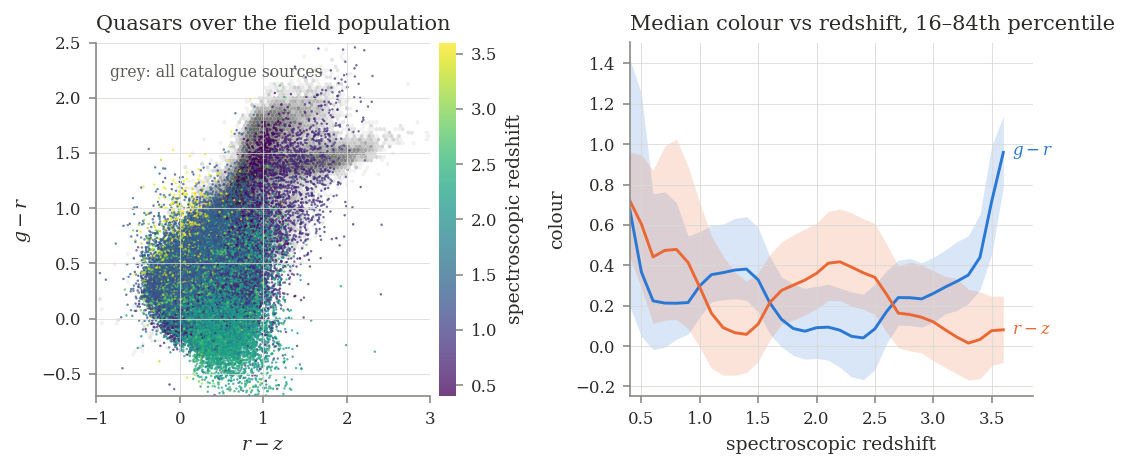
\includegraphics[width=\textwidth]{../../plots/method/fig1_qso_locus.png}
\caption{DESI DR1 quasars in Legacy Surveys DR9 photometry. \emph{Left:} the
quasar locus, coloured by spectroscopic redshift, over the density of all
catalogue sources in the same field (grey). The quasar and field populations
overlap substantially --- discrimination comes from where in the plane an object
sits, not from a clean separation. \emph{Right:} median colour against redshift
with the $16$--$84$th percentile band. The track is strongly non-monotonic,
which is the property that shapes the choice of model in
\S\ref{sec:slices}.}
\label{fig:locus}
\end{figure}

\subsection{Extreme deconvolution}
\label{sec:xd}

Each object's colours are measured with its own heteroscedastic, correlated
error. Fitting a mixture to the observed points would recover the locus
\emph{convolved} with those errors, which is systematically too wide, and the
width is exactly what discriminates. We therefore fit the \emph{intrinsic}
distribution by extreme deconvolution \citep{bovy2011xd}: a Gaussian mixture
%
\begin{equation}
p(\mathbf{v}) = \sum_{k} \alpha_k\,
\mathcal{N}(\mathbf{v}\mid\boldsymbol{\mu}_k,\mathbf{V}_k)
\label{eq:mixture}
\end{equation}
%
whose components are convolved with each observation's covariance
$\mathbf{S}_i$ during fitting, so that the density of the \emph{observed} value
is evaluated with $\mathbf{V}_k+\mathbf{S}_i$. The EM update is given in
Appendix~\ref{app:xd}. Figure~\ref{fig:deconv} tests this on real quasar
colours by injecting noise of known size: the deconvolved width is recovered to
within $7\%$ after the observed width has more than doubled, while an ordinary
mixture tracks the broadened distribution exactly. The correction matters most
where the measurement error approaches the intrinsic width of the locus, which
in these data is the faint end.

\begin{figure}[t]
\centering
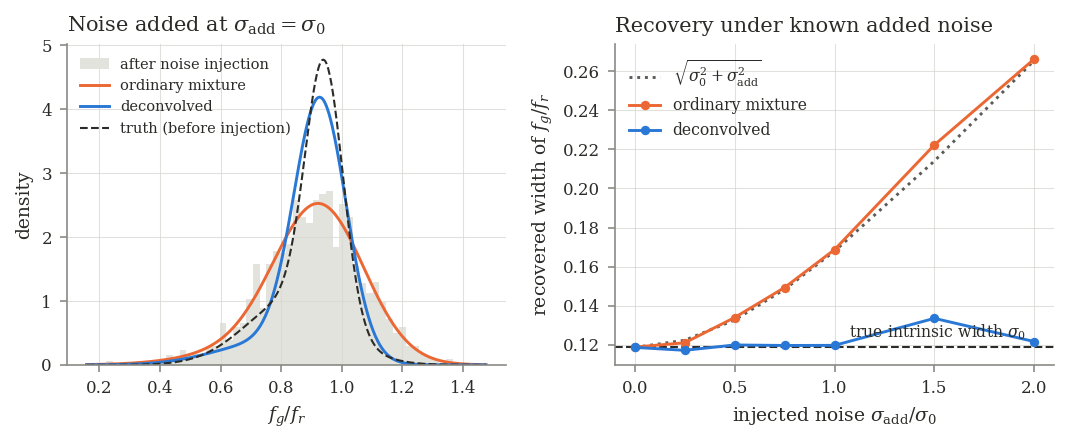
\includegraphics[width=\textwidth]{../../plots/method/fig4_deconvolution.png}
\caption{Deconvolution tested by controlled noise injection on real quasar
colours. Bright quasars near $z=1.8$ ($N=1536$, $r<20$) have negligible
measurement errors, so their fitted width $\sigma_0=0.119$ is effectively the
intrinsic one. Gaussian noise of known size is then added and the models
refitted. \emph{Left:} at $\sigma_{\rm add}=\sigma_0$ the deconvolved mixture
(blue) recovers the pre-injection truth (dashed) while the ordinary mixture
(orange) is visibly broadened. \emph{Right:} the ordinary mixture follows
$\sqrt{\sigma_0^2+\sigma_{\rm add}^2}$ exactly, as it must, reaching $0.267$ at
$\sigma_{\rm add}=2\sigma_0$; extreme deconvolution stays flat, returning
$0.127$ --- within $7\%$ of the truth after the observed width has more than
doubled.}
\label{fig:deconv}
\end{figure}

\subsection{Conditional slices rather than a joint mixture}
\label{sec:slices}

There are two natural ways to make the mixture redshift-dependent.

The first, following XDQSOz \citep{bovy2012xdqsoz}, fits a single mixture to the
joint vector $[\cvec,z]$ and conditions analytically on $z$. It is elegant and
gives a closed-form photometric redshift distribution. It has two properties
that are awkward here. Within a component the colour--redshift relation is
\emph{linear}, so representing the strongly curved track of
Figure~\ref{fig:locus} requires components narrow in $z$, and the required
number is set by the curvature rather than by the data volume. Second,
conditioning on $z$ reweights components by their $z$-marginal, which is the
redshift distribution of the \emph{training sample} --- that is, of the
spectroscopic target selection. The conditional density is still correct, but
the redshift prior enters implicitly.

The second, which we adopt as the default, fits an independent deconvolved
mixture in each of a set of overlapping redshift slices and interpolates
linearly in density between neighbouring slice centres:
%
\begin{equation}
p(\cvec\mid Q,z) = (1-w)\,p_{j}(\cvec) + w\,p_{j+1}(\cvec),
\qquad
w = \frac{z-z_j}{z_{j+1}-z_j}.
\label{eq:slices}
\end{equation}
%
Because each $p_j$ is normalised over colour space, \eqref{eq:slices} is a
normalised density for any $z$, and the training sample's redshift distribution
\emph{between} slices cannot leak into it. It does not follow that no
redshift-selection effect survives: a slice of finite width estimates the
colour distribution averaged over the training redshifts \emph{within} that
slice, so a strongly varying targeting rate inside a slice still biases it, and
colour-dependent selection affects both this and the joint construction
equally. Narrower slices reduce the residual at the cost of statistics.

What the slice construction does buy is that the redshift resolution becomes an
explicit, tunable quantity, and that the redshift prior is supplied separately
and visibly as $\Sq(z,m)$ rather than inherited. Figure~\ref{fig:slices} shows the fitted conditional at three
redshifts.

Both backends implement the same density interface, but they are not yet
interchangeable in the scorer, which calls a slice-specific method to reuse
precomputed per-slice densities. Using the joint model for candidate scoring
needs that path generalised first. Which predicts held-out quasar colours better
remains an empirical question, to be settled by measurement rather than by the
argument above.

\begin{figure}[t]
\centering
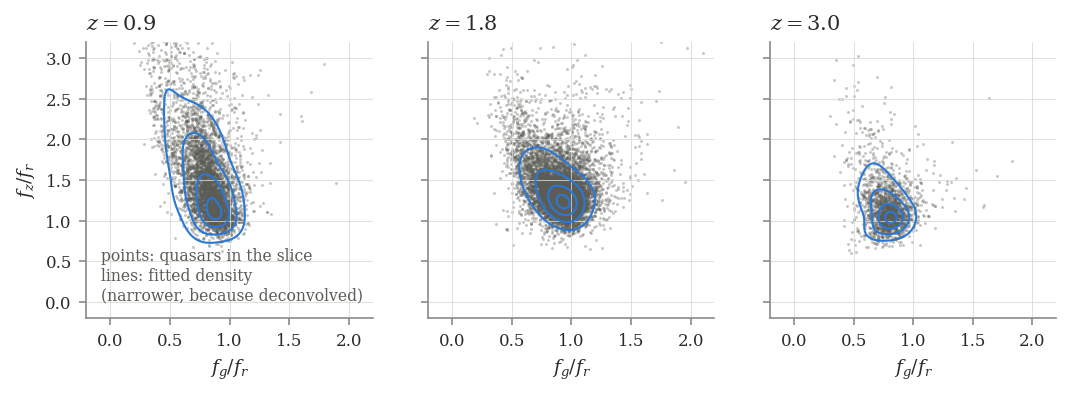
\includegraphics[width=\textwidth]{../../plots/method/fig2_model_slices.png}
\caption{The fitted conditional density $p(\cvec\mid Q,z)$ at three redshifts
(contours), with the quasars in each slice (points). The locus translates and
changes shape with redshift; each slice is a separate deconvolved mixture, so no
linear colour--redshift relation is imposed. The contours are visibly tighter
than the scatter of the points because the model is the \emph{deconvolved}
density, while the points carry their measurement errors
(\S\ref{sec:xd}). Note also how much the three loci overlap: this is the
origin of the weak redshift discrimination quantified in
\S\ref{sec:howmuch}.}
\label{fig:slices}
\end{figure}

\subsection{Missing bands}

A Gaussian mixture marginalises exactly over unobserved dimensions: one deletes
the corresponding rows and columns of every component covariance and of the
observation's covariance, and evaluates the resulting lower-dimensional density.
No imputation is involved, and the result is the correct likelihood of what was
actually measured. The practical consequence is that a candidate lacking one
band is still scored, with correspondingly weaker discrimination, rather than
being dropped or given a survey-median colour.

\section{The background model}
\label{sec:background}

The competing density $p(\cvec\mid B,m,\ell,b)$ is built from the imaging
catalogue itself, over the same footprint and with the same quality definition
applied to the candidates. No star/galaxy separation is imposed, because
imposing one would require a selection function we do not have, whereas the
unfiltered catalogue \emph{is} the population a chance projection draws from.

\paragraph{A known violation of disjointness.} The formalism of
\S\ref{sec:hypotheses} treats $\Hfield$ and $\Hbkg$ as mutually exclusive, but
the background sample as currently built does not exclude spectroscopic
quasars, so quasars are counted in both. They are a tiny fraction of all
catalogue sources, which is \emph{not} an argument that the effect is small:
what matters is their fraction in quasar-like colour space, which is exactly
where the same-redshift hypothesis is being tested. Removing them requires a
crossmatch against the quasar catalogue. Until that is done and the size of the
effect measured, the background is over-dense at quasar colours and
$p_{\rm same}$ is correspondingly conservative there.

The density depends on position, through Galactic structure and reddening, and
on magnitude, through which populations are reachable at a given depth. We
therefore fit a deconvolved mixture per (HEALPix cell, magnitude bin) and pool
sparse cells towards coarser ones:
%
\begin{equation}
p = a_\ell\,p_{\rm cell} + (1-a_\ell)\bigl[
      a_p\,p_{\rm parent} + (1-a_p)\,p_{\rm global}\bigr],
\qquad a = \frac{n}{n+n_0},
\label{eq:hierarchy}
\end{equation}
%
with a pooling constant $n_0$ that is \emph{intended} to be tuned on held-out
sky blocks rather than fixed in code. It is not yet: the tuning routine holds
out whole cells at the same resolution as the parent level, so every validation
object falls back to the global model and its score carries no information about
$n_0$. The figures in this note therefore use a fixed $n_0=500$, and the tuning
must be repaired before any calibrated number depends on it. HEALPix is used in
the nested scheme, so a parent cell is a bit shift,
and in Galactic coordinates, which is the frame the structure lives in. Each
scored object records the weight its own cell received, so a number that came
from the pooled model is distinguishable from one that came from local data.

Figure~\ref{fig:densities} shows the two class-conditional densities in the same
plane and the resulting colour Bayes factor. The populations overlap; the method
does not pretend otherwise, and the Bayes factor is smoothly varying rather than
a decision boundary.

\begin{figure}[t]
\centering
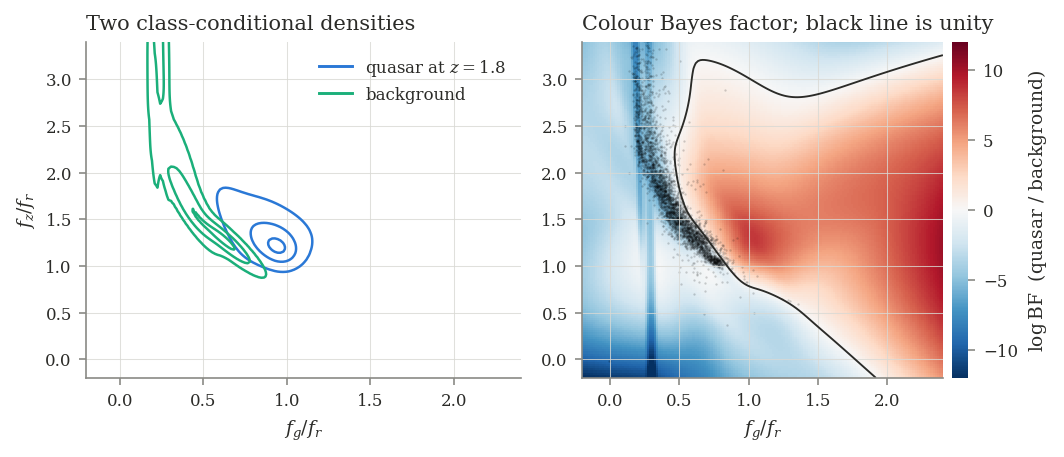
\includegraphics[width=\textwidth]{../../plots/method/fig3_two_densities.png}
\caption{\emph{Left:} the quasar density at $z=1.8$ and the local background
density, both fitted to real data, in the same feature plane. \emph{Right:} the
colour Bayes factor \eqref{eq:bf}; the black contour is $\mathrm{BF}=1$, and
black points are real catalogue sources at the relevant magnitude. Most of the
field population sits where the Bayes factor strongly disfavours the quasar
hypothesis, but the two loci are not disjoint.}
\label{fig:densities}
\end{figure}

\section{Surface densities}
\label{sec:priors}

The two surface densities must be measured over footprints whose selection and
usable area are known, and the same cuts must be applied to the candidates. The
illustration in this note does not fully meet that standard: for speed it draws
quasars from a $12^\circ$ cone and background sources from a $1^\circ$ cone at
the same centre, and applies a mask-bit cut without a mask-corrected area. Each
density uses its own area, so the arithmetic is consistent, but matched
selection and area should be read as requirements of the method rather than as
properties these particular figures demonstrate.

\paragraph{Background.} $\Sb(m,\ell,b)$ is estimated by counting the imaging
catalogue into the same (cell, magnitude) bins and dividing by the \emph{usable}
area after masking. That area must be supplied; the implementation refuses to
run without it. The reason is not pedantry: an earlier version of the figure
pipeline defaulted to the nominal HEALPix pixel area, $53.7\,{\rm deg}^2$ at
nside~8, for a background cone of $3.14\,{\rm deg}^2$, understating $\Sb$ by a
factor of $17$ and inflating every quasar posterior by the same factor. Cells
that were surveyed but happen to hold no object in a magnitude bin must also
stay in the denominator, or sparse bins are biased high. The masking is applied
identically to the candidates, so the two are consistent by construction.

\paragraph{Quasars.} $\Sq(z,m)$ requires more care, because a spectroscopic
quasar catalogue's redshift histogram is a targeting selection function, not a
quasar population. We estimate
%
\begin{equation}
\Sq(z,m) = \frac{N(z,m)}{A\,\Delta z\,\Delta m\,C(z,m)},
\label{eq:sigma_q}
\end{equation}
%
with $A$ the surveyed area and $C\le1$ the spectroscopic completeness. The
default is $C=1$, which understates the quasar density everywhere.

That does \emph{not} make $p_{\rm same}$ a lower bound, and an earlier version
of this note wrongly said it did. The bound holds only if completeness is
independent of redshift, so that correcting it scales $\lambda_{\rm same}$ and
$\lambda_{\rm field}$ together and only the fixed background dilutes. If
completeness is worse away from $z_0$ than at it, correcting it raises the field
term more and the posterior \emph{falls}: intensities $(1,1,1)$ give $1/3$,
while a correction that multiplies only the field term by $100$ gives $1/102$.
$C=1$ is a declared, reproducible default, not a conservative one. Where no defensible prior exists at all, the
implementation returns the Bayes factor and leaves the posterior fields null
with a status code, rather than substituting a class fraction.

\section{The redshift window is a multiplicative constant}
\label{sec:window}

This section contains the main methodological point.

\subsection{The tension}

A physically motivated pair window is of order $\pm2000\kms$. At $z_0=1.4$ that
is
%
\begin{equation}
\Delta z = (1+z_0)\,\frac{\Delta v}{c}
         = 2.4\times\frac{2000}{299792.458} = 0.016 .
\end{equation}
%
Broadband colours constrain a quasar redshift far more loosely, and often to a
multimodal distribution rather than a single peak --- which is why XDQSOz
produces a redshift \emph{PDF} in the first place \citep{bovy2012xdqsoz}.
Measured on $1500$ real DESI quasars with the model of \S\ref{sec:qso}, the
median posterior width $\sigma_z\approx0.6$ (16--84th percentile $0.36$--$0.78$; 68\% credible interval $\approx0.71$ wide). The median distance from the posterior mean to the
spectroscopic redshift is $0.28$, so the point estimate is better than the
posterior width alone suggests; but it is the \emph{width} that governs how
much probability a narrow window can capture. Rather than quote a ratio --- which
would compare a standard deviation with a window width, two different summaries
--- note the two numbers directly: at $z_0=1.8$ the window spans $0.037$ in
redshift while the posterior has a standard deviation of $0.6$. For a unimodal
posterior of that width, a window of that span captures of order two per cent of
the probability.
Figure~\ref{fig:window} shows this for three real quasars.

The arithmetic consequence is unavoidable: almost all of a candidate's quasar
intensity falls outside the window, so
$\lambda_{\rm field}\gg\lambda_{\rm same}$ and $p_{\rm same}$ is small even for
an object sitting exactly on the locus at exactly the right redshift. This is
not a defect of the method. It is the correct answer to the question as posed,
and it means the question as posed is not the one colours can answer.

\begin{figure}[t]
\centering
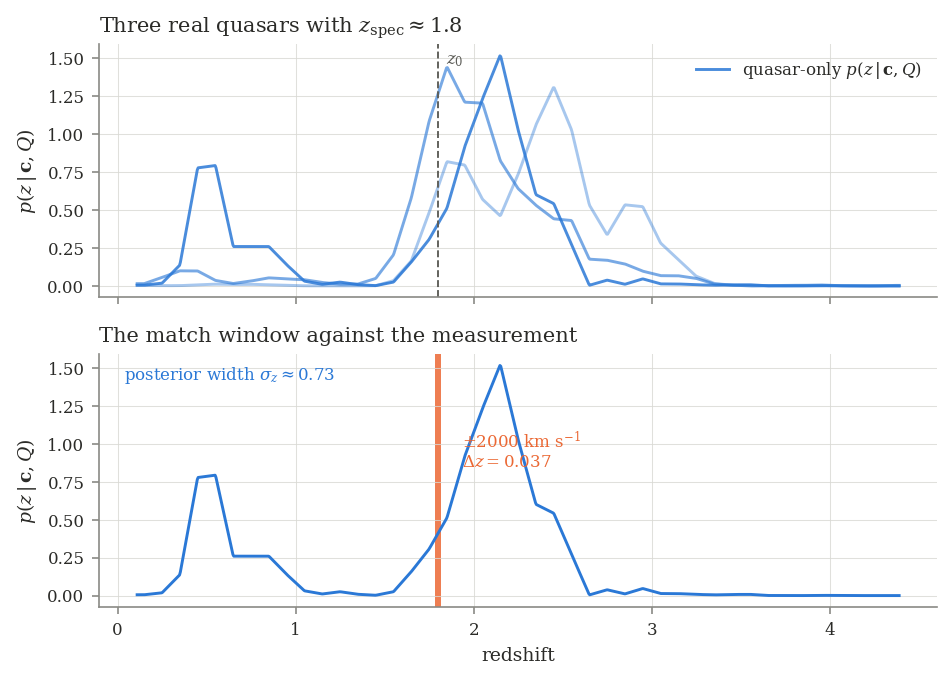
\includegraphics[width=0.86\textwidth]{../../plots/method/fig5_window.png}
\caption{\emph{Top:} quasar-only redshift posteriors $p(z\mid\cvec,Q)$ for three
real DESI quasars with $z_{\rm spec}\approx1.8$, showing the width and the
secondary solutions that broadband colours cannot resolve. \emph{Bottom:} the
same posterior with a $\pm2000\kms$ window drawn to scale. The window is the
narrow orange band. The width quoted on the panel is for \emph{this} object,
which is better constrained than most; across $1500$ quasars the median width
is $\sigma_z\approx0.6$ (\S\ref{sec:window}). Note that this is the quasar-only posterior under a \emph{flat} redshift
prior; $p_{\rm same}$ integrates the same window against
$\Sigma_Q(z,m)\,p(\cvec\mid Q,z)$ instead. The panel shows the scale of the
mismatch between window and measurement, which is what makes $p_{\rm same}$
small, not the quantity itself.}
\label{fig:window}
\end{figure}

\subsection{Which uncertainty is the problem}
\label{sec:whichsigma}

It is worth being explicit about \emph{whose} redshift is uncertain, because
the two quantities differ by three orders of magnitude and only one of them
matters.

\begin{center}
\begin{tabular}{lrr}
\toprule
 & $\Delta z$ at $z=1.8$ & relative \\
\midrule
primary's spectroscopic error        & $0.0004$ & $1\times$ \\
$\pm2000\kms$ window (half-width)    & $0.019$  & $49\times$ \\
companion's photometric width        & $0.6$    & $1579\times$ \\
\bottomrule
\end{tabular}
\end{center}

The primary is a spectroscopic object: the median DESI DR1 quasar redshift
error is $0.0004$, or $43\kms$. It is known some $1600$ times better than the
companion, and contributes essentially nothing to the blur. The entire
difficulty sits on the companion, which has no spectrum. A perfectly known
primary redshift does not help, because it is not the uncertain quantity.

What the primary's precision \emph{does} buy is that
$p(\cvec\mid Q,z_0)$ is evaluated at a sharp point rather than marginalised
over a second unknown redshift. That is a real simplification, and it is what
makes the calculation tractable at all. The primary's error enters by \emph{marginalising} the window over it, which
smooths the window's edges while conserving its area; a top hat becomes a
difference of normal CDFs. An earlier implementation instead replaced the
half-width by $\sqrt{s^2+\sigma_{\rm primary}^2}$, which increased the area, so
a less certain primary produced a larger expected number of same-redshift
quasars --- uncertainty about where the window sits cannot create companions.

One caveat for practice: the $43\kms$ above is a \emph{pipeline statistical}
error. Quasar systemic redshifts derived from broad lines, and C\,\textsc{iv}
in particular, carry known systematic offsets that are a non-trivial fraction
of a pair window. Where the window matters, \texttt{z\_primary\_err} should be
set to a systemic uncertainty measured for the redshift estimator actually
used, not to the pipeline value.

\subsection{What sets the companion's width}
\label{sec:whatsets}

To first order,
%
\begin{equation}
\sigma_z \;\approx\;
\frac{\text{scatter of colour at fixed } z}
     {\left|\mathrm{d}(\text{colour})/\mathrm{d}z\right|} ,
\label{eq:sigmaz}
\end{equation}
%
a ratio between how fast the locus moves and how wide it is. Measured on our
quasars near $z=1.8$:

\begin{center}
\begin{tabular}{lrrr}
\toprule
colour & $|\mathrm{d}C/\mathrm{d}z|$ & scatter at fixed $z$ & implied $\sigma_z$ \\
\midrule
$g-r$ & $0.356$ & $0.219$ & $0.62$ \\
$r-z$ & $0.402$ & $0.229$ & $0.57$ \\
\bottomrule
\end{tabular}
\end{center}

Combining the two as if independent gives $0.42$; the full posteriors give
$0.60$, the difference being the correlation between colours and the
multimodality created where the locus doubles back on itself.

The practical reading of \eqref{eq:sigmaz} is that the denominator, not the
numerator, is the lever. At bright magnitudes the scatter is dominated by
\emph{intrinsic} quasar-to-quasar diversity rather than measurement error ---
which is exactly what the injection test of Figure~\ref{fig:deconv}
establishes, with an intrinsic $\sigma_0=0.119$ in $f_g/f_r$ where the
measurement error is negligible. Deeper imaging in the same bands therefore
buys little. Improving the redshift constraint requires bands in which quasar
colour changes \emph{faster} with redshift: a $u$ band spanning the Lyman
break, or a narrow band tracking a strong emission line.

\subsection{Factorising the window out}

The resolution is to stop treating the window as part of the model. Because it
is much narrower than the scale on which
$\Sq(z,m)\,p(\cvec\mid Q,z)$ varies, \eqref{eq:lam_same} becomes
%
\begin{equation}
\lambda_{\rm same} \simeq
\Delta Z_{\rm eff}\;\Sq(z_0,m)\;p(\cvec\mid Q,z_0),
\qquad
\Delta Z_{\rm eff} \equiv \int W(z\mid z_0)\,\dd z ,
\label{eq:narrow}
\end{equation}
%
with an error of order $(\Delta z/\sigma_z)^2$. The window area
$\Delta Z_{\rm eff}$ is $2s$ for a top hat of half-width $s$ and
$\sqrt{2\pi}\,s$ for a Gaussian, and is evaluated in closed form.

The step that makes this clean is the denominator. Since $\Hsame$ and $\Hfield$
\emph{partition} the quasar intensity,
%
\begin{equation}
\lambda_{\rm same}+\lambda_{\rm field}+\lambda_{\rm bkg}
= \Lambda_{Q,{\rm tot}} + \lambda_{\rm bkg}
\qquad\text{for \emph{any} window,}
\label{eq:partition}
\end{equation}
%
where $\Lambda_{Q,{\rm tot}}=\int\Sq(z,m)\,p(\cvec\mid Q,z)\,\dd z$. Defining
%
\begin{equation}
\boxed{\;
R \;\equiv\;
\frac{\Sq(z_0,m)\;p(\cvec\mid Q,z_0)}
     {\Lambda_{Q,{\rm tot}} + \lambda_{\rm bkg}}
\;}
\qquad [\text{redshift}^{-1}]
\label{eq:R}
\end{equation}
%
and combining \eqref{eq:narrow}--\eqref{eq:partition} with
\eqref{eq:posterior} gives
%
\begin{equation}
p_{\rm same} = R\;\Delta Z_{\rm eff},
\label{eq:linear}
\end{equation}
%
a linear relation, not an odds transformation.

Two cautions about what this does and does not establish, both of which an
earlier version of this note got wrong.

First, \eqref{eq:partition} is exact, but \eqref{eq:narrow} is an
approximation. Writing $f(z)=\Sigma_Q(z,m)p(\cvec\mid Q,z)$, the exact
statement is
%
\begin{equation}
p_{\rm same}
= R(z_0)\,\Delta Z_{\rm eff}
+ \frac{\int W(z)\,[f(z)-f(z_0)]\,\dd z}{D},
\qquad D = \int f\,\dd z + \lambda_{\rm bkg},
\end{equation}
%
so the linear relation holds to the extent that $f$ is flat across the window.
The leading relative correction is $f''(z_0)s^2/[6f(z_0)]$ for a top hat. Calling
that $O((s/\sigma_z)^2)$ assumes the posterior width measures local curvature,
which a multimodal posterior need not satisfy; at a cusp --- and both the
likelihood and the prior are interpolated piecewise-linearly --- the error is
instead $O(s)$.

Second, in the implementation $R$ is computed as the \emph{window-averaged}
intensity, $R = p_{\rm same}/\Delta Z_{\rm eff}$. Equation~\eqref{eq:linear}
therefore holds for the reported number \emph{by construction}; it is a
definition, not a derived result. The substantive claim is the separate one that
$R$ does not depend on the window, and that holds only in the narrow limit.
Figure~\ref{fig:factorisation} tests it on a real object: over a factor of ten
in window width $R$ moves by well under a per cent. For a window comparable to
$\sigma_z$ it is a genuine average and does vary.

\begin{figure}[t]
\centering
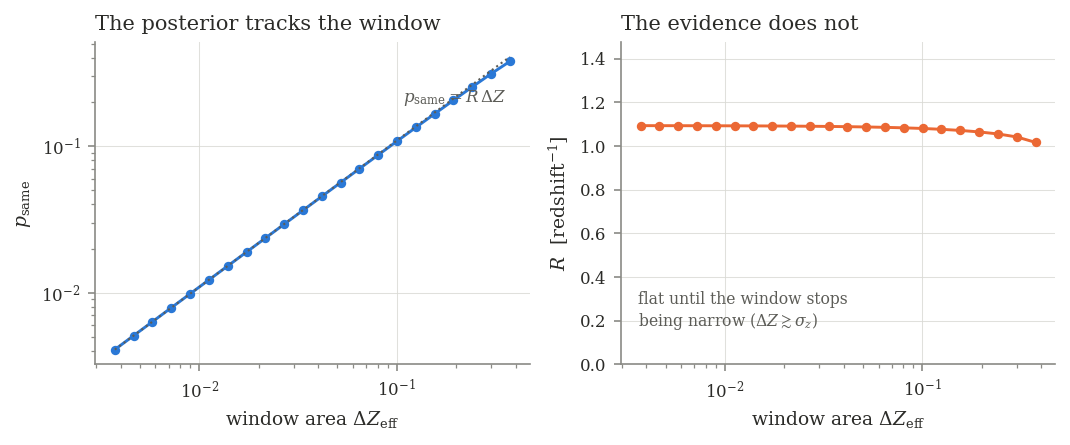
\includegraphics[width=\textwidth]{../../plots/method/fig6_factorisation.png}
\caption{The factorisation, on a real quasar. \emph{Left:} $p_{\rm same}$ is
proportional to the window area over more than a decade, exactly as
\eqref{eq:linear} requires; the dotted line is $R\,\Delta Z$ with $R$ taken from
the narrowest window. \emph{Right:} $R$ itself is flat, departing only when the
window stops being narrow compared with $\sigma_z$ and the approximation in
\eqref{eq:narrow} is no longer appropriate.}
\label{fig:factorisation}
\end{figure}

\subsection{Consequences}

\begin{enumerate}
\item \textbf{Rank on $R$.} It is the window-free evidence, so two people can
      compare candidates without first agreeing on a window, and it is not
      compressed towards zero the way $p_{\rm same}$ is.
\item \textbf{Never quote $p_{\rm same}$ without its window.} The two travel
      together in every output row, as \texttt{p\_sameq} and
      \texttt{dz\_match\_eff}.
\item \textbf{Never integrate a velocity window on the main redshift grid.}
      $\Delta Z_{\rm eff}=0.03$ on a grid of step $0.01$ spans two or three
      points, and a sampled top hat there quantises the answer in units of the
      grid step --- up to $20\%$ in the regime this project works in. An
      earlier implementation switched between that integral and the closed form
      \eqref{eq:narrow} on a grid-resolution test, which merely chose between
      two inaccurate branches and also counted window area lying outside the
      trained redshift range. The window integral is now done on its own dense
      sub-grid, over the intersection of the window with the model's support:
      one path, exact at any width, with no invented area at the edges.
\item \textbf{Widening the window does not improve the answer.} It changes the
      question. With $R$ reported separately there is no incentive to.
\end{enumerate}

\subsection{How much discrimination is actually available}
\label{sec:howmuch}

Figure~\ref{fig:separation} evaluates $R$ against a primary at $z_0=1.8$ for
three real populations, and the result is worth stating plainly because it sets
expectations for the whole programme.

\begin{center}
\begin{tabular}{lr}
\toprule
population & median $\log R$ \\
\midrule
quasars at $z\approx z_0$        & $-0.3$ \\
quasars at other redshifts       & $-2.6$ \\
random catalogue sources         & $-14.3$ \\
\bottomrule
\end{tabular}
\end{center}

Two very different gaps. Against the field population the statistic is
decisive: $e^{14.0}\approx10^{6}$. Against \emph{quasars at the wrong
redshift} it is worth a factor of about $10$.

That asymmetry is not a defect of the estimator; it is a statement about the
information content of $grz+W1W2$ photometry. These bands identify quasars
very well and locate them in redshift only weakly --- which is visible directly
in Figure~\ref{fig:slices}, where the conditional loci at $z=0.9$, $1.8$ and
$3.0$ overlap substantially, and in the posterior widths of
Figure~\ref{fig:window}.

The consequences for practice are concrete:

\begin{itemize}
\item \textbf{What this method delivers reliably is a quasar classification},
      not a redshift match. A companion with high $R$ is very likely a quasar;
      whether it is at $z_0$ is a much weaker inference.
\item \textbf{The field-quasar hypothesis is therefore not a refinement but
      the dominant competing explanation}, which is precisely why a
      quasar-versus-star calculation would be misleading here rather than
      merely incomplete.
\item \textbf{Improving redshift discrimination plausibly requires more
      information}: a $u$ band or a narrow band bracketing a strong line,
      variability, or ultimately spectroscopy. This is a reading of
      \eqref{eq:sigmaz} together with the injection test, not a proven bound ---
      the numbers come from one untuned model on one sky patch, evaluated in
      sample, and a difference between population medians establishes neither
      purity nor an information limit. The modular likelihood structure is
      designed so such a term can be added as a factor rather than by rewriting
      the inference.
\end{itemize}

\begin{figure}[t]
\centering
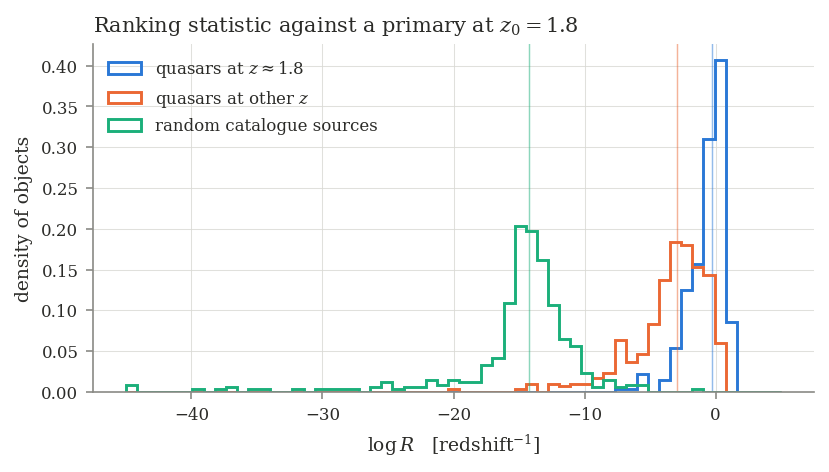
\includegraphics[width=0.74\textwidth]{../../plots/method/fig7_separation.png}
\caption{The ranking statistic evaluated against a primary at $z_0=1.8$, for
real quasars at that redshift ($|z-z_0|<0.05$), real quasars at other redshifts
($|z-z_0|>0.6$), and random catalogue sources. Vertical lines mark the medians.
Two limits of this comparison: the ``same'' class extends to $2.7$ times the
window half-width, so not all of it lies inside the window being scored; and
nothing populates the gap between $0.05$ and $0.6$, which is where
discrimination is genuinely hardest; and these objects were used in training.
The quasar populations separate from the field by $\sim\!14$ natural logarithms
but from \emph{each other} by only $\sim\!2.3$: $grz+W1W2$ photometry
identifies quasars far better than it locates them in redshift
(\S\ref{sec:howmuch}). The figure shows the statistic's dynamic range, not an
operating characteristic.}
\label{fig:separation}
\end{figure}

\section{What the scorer returns}
\label{sec:outputs}

Every candidate produces a record separating evidence from posterior, with a
status code and quality flags rather than a silent number.

\begin{center}
\begin{tabular}{lp{9.4cm}}
\toprule
\texttt{loglike\_qso\_zprimary} & $\log p(\cvec\mid Q,z_0)$; a likelihood, not a
probability \\
\texttt{loglike\_bkg} & $\log p(\cvec\mid B,m,\ell,b)$ \\
\texttt{log\_bayes\_factor\_qz\_bkg} & \eqref{eq:bf}; independent of both
surface densities \\
\texttt{p\_zmatch\_given\_qso} & $P(z\in W\mid\cvec,Q)$; conditional on being a
quasar at all \\
\texttt{z\_phot\_mode} & mode of the quasar-only redshift posterior \\
\texttt{log\_r\_per\_unit\_z} & $\log R$ from \eqref{eq:R}; the ranking
statistic, window-free in the narrow limit (\S\ref{sec:window}) \\
\texttt{dz\_match\_eff} & $\Delta Z_{\rm eff}$ \emph{actually used}, i.e. the
window area inside the model's support, so that
$p_{\rm same}=R\,\Delta Z_{\rm eff}$ \\
\texttt{log\_lambda\_sameq}, \texttt{\_fieldq}, \texttt{\_bkg} &
\eqref{eq:lam_same}--\eqref{eq:lam_bkg} in logs \\
\texttt{p\_sameq} & \eqref{eq:posterior}, the three-hypothesis posterior \\
\texttt{p\_sameq\_vs\_bkg} & the two-hypothesis number; ignores field quasars \\
\texttt{qso\_ood\_sigma} & distance to the nearest training component, in
$\sigma$ \\
\texttt{background\_local\_weight} & $a_\ell$ from \eqref{eq:hierarchy}; zero
means a pooled model \\
\texttt{background\_density\_level} & 0 local, 1 parent, 2 global \\
\texttt{n\_bands\_used} & usable feature dimensions for this object \\
\texttt{status}, \texttt{quality\_flags} & why a value is missing, and what is
suspect about one that is not \\
identification & \texttt{candidate\_id}, \texttt{primary\_id},
\texttt{ref\_mag}, \texttt{photometric\_system},
\texttt{model\_manifest\_id} --- so a number can be traced back to the model
and the data that produced it \\
\bottomrule
\end{tabular}
\end{center}

\section{Validation design}
\label{sec:validation}

Nothing above is evidence that the method works. That requires a labelled
sample, and one exists: pairs in which \emph{both} members have spectra. Around
each spectroscopic quasar we take every companion that also has a spectrum and
label it by what that spectrum says --- a quasar at the same redshift, a quasar
at a different redshift, or something else. The \emph{labels} are spectroscopic and so independent of the colours being
scored. The \emph{inclusion} of an object in the sample is not: DESI targets
quasars with a classifier built on these very photometric features, so the
labelled set is a colour-selected subset of the sky. Stratifying by magnitude
and latitude does not correct targeting, fibre assignment or redshift-success
selection, and calibration measured on this sample transfers only to candidates
drawn the same way. Quantifying that is part of the validation, not a caveat to
be noted and passed over.

From DESI DR1, at separations of $3$--$20''$, this yields approximately $1600$
confirmed same-redshift pairs and $8400$ projected quasar--quasar pairs, plus
every confirmed star or galaxy companion. Calibration must then be assessed
\emph{stratified} by separation, blending diagnostic, magnitude, Galactic
latitude and redshift, because the prevalence of each class changes strongly
along all of them.

Two cautions were established while assembling this sample.

\paragraph{De-duplicate by position, not by identifier.} Of the $10\,636$
DESI quasar ``pairs'' closer than $3''$, $9577$ lie within $0.5''$ with
identical redshifts: they are the same physical object entered twice under two
target identifiers. The catalogue's own primary-object flag does not remove
them. Training on such a sample silently up-weights repeated objects.

\paragraph{Training-set selection is not neutral.} DESI quasar targeting uses a
random forest on the very Legacy Surveys colours we model, so the training set
gives $p(\cvec\mid Q,z,\text{selected by DESI})$. The mitigation is to report
held-out likelihood separately on an independently selected sample --- SDSS
DR16Q \citep{lyke2020dr16q}, whose targeting channels differ --- and to treat a
large gap as a selection-bias warning rather than a curiosity.

\section{Scope and limitations}
\label{sec:limitations}

\paragraph{Blending is the binding constraint.} Below a few arcseconds the
Legacy Surveys model fit divides flux between overlapping sources, so the two
colour vectors are neither independent nor individually reliable, and a
probability computed from them describes the deblender rather than the sky. The
current pipeline therefore scores cleanly deblended companions only, enforced by
an explicit separation floor and blending limit; a candidate lacking those
measurements is treated as blended, because it cannot be certified clean without
them. Closer pairs require image-level forced photometry, which is separate
work.

\paragraph{$p_{\rm same}$ is not the probability of a physical pair.} It is a
classification posterior under the adopted population priors. A physical-pair
calculation additionally requires conditioning the quasar intensity on angular
separation from the primary through small-scale quasar clustering
\citep{hennawi2006,eftekharzadeh2017}. That layer is deliberately separate, must
come from an externally specified measurement used inside its documented regime,
and must be reported separately from the photometric posterior.

\paragraph{Unused evidence.} Gaia parallax and proper motion settle the question
outright for bright companions and are available in the same catalogue; WISE
photometry is the single strongest star/quasar discriminant but has a $\sim6''$
beam and is therefore the most blend-contaminated. Running optical-only and
optical$+$WISE models side by side makes their disagreement a blending
diagnostic. Variability is not uniformly available over the footprint and is out
of scope here.

\appendix

\section{Gaussian identities used}
\label{app:gauss}

For a mixture \eqref{eq:mixture} over a partitioned vector
$\mathbf{v}=[\mathbf{a},\mathbf{b}]$ and an observation
$\mathbf{b}=\mathbf{y}$ with covariance $\mathbf{S}_y$, the conditional is
again a mixture, with weights
%
\begin{equation}
w_k \propto \alpha_k\,
\mathcal{N}\bigl(\mathbf{y}\mid\boldsymbol{\mu}_{b,k},
\mathbf{V}_{bb,k}+\mathbf{S}_y\bigr),
\end{equation}
%
and components
%
\begin{align}
\boldsymbol{\mu}_{a\mid y,k} &= \boldsymbol{\mu}_{a,k}
  + \mathbf{V}_{ab,k}\bigl(\mathbf{V}_{bb,k}+\mathbf{S}_y\bigr)^{-1}
    (\mathbf{y}-\boldsymbol{\mu}_{b,k}),\\
\mathbf{V}_{a\mid y,k} &= \mathbf{V}_{aa,k}
  - \mathbf{V}_{ab,k}\bigl(\mathbf{V}_{bb,k}+\mathbf{S}_y\bigr)^{-1}
    \mathbf{V}_{ba,k}.
\end{align}
%
The appearance of $\mathbf{S}_y$ in the weights is how an uncertain primary
redshift broadens the match rather than being ignored. Marginalising over a
subset of dimensions simply deletes the corresponding rows and columns. In the
implementation no inverse is ever formed: every quadratic form and log
determinant comes from a Cholesky factor, and all densities are computed in log
space with \texttt{logsumexp}.

\section{The extreme-deconvolution update}
\label{app:xd}

For observation $i$ with observed sub-vector $\mathbf{w}_i$, noise covariance
$\mathbf{S}_i$, and component $j$, write $O$ for the observed dimensions and
%
\begin{align}
\mathbf{T}_{ij} &= \mathbf{V}_j^{OO} + \mathbf{S}_i, &
q_{ij} &\propto \alpha_j\,\mathcal{N}\bigl(\mathbf{w}_i\mid
        \boldsymbol{\mu}_j^{O},\mathbf{T}_{ij}\bigr), \\
\mathbf{b}_{ij} &= \boldsymbol{\mu}_j
  + \mathbf{V}_j^{\cdot O}\mathbf{T}_{ij}^{-1}
    \bigl(\mathbf{w}_i-\boldsymbol{\mu}_j^{O}\bigr), &
\mathbf{B}_{ij} &= \mathbf{V}_j
  - \mathbf{V}_j^{\cdot O}\mathbf{T}_{ij}^{-1}\mathbf{V}_j^{O\cdot},
\end{align}
%
with the M step
%
\begin{equation}
\alpha_j = \frac{1}{N}\sum_i q_{ij},
\quad
\boldsymbol{\mu}_j = \frac{\sum_i q_{ij}\mathbf{b}_{ij}}{\sum_i q_{ij}},
\quad
\mathbf{V}_j = \frac{\sum_i q_{ij}\bigl[\mathbf{B}_{ij}
   + (\mathbf{b}_{ij}-\boldsymbol{\mu}_j)
     (\mathbf{b}_{ij}-\boldsymbol{\mu}_j)^{\!\top}\bigr]}{\sum_i q_{ij}} .
\end{equation}
%
With $\mathbf{S}_i=0$ and no missing dimensions this reduces exactly to ordinary
Gaussian-mixture EM. Restricting $O$ per object is how missing bands are handled
without projection matrices. Sample weights multiply every sum, which is where
selection-function weights would enter.

\begin{thebibliography}{9}

\bibitem[Bovy et al.(2011)]{bovy2011xd}
Bovy J., Hogg D.~W., Roweis S.~T., 2011,
\emph{Extreme deconvolution: inferring complete distribution functions from
noisy, heterogeneous and incomplete observations},
\url{https://arxiv.org/abs/0905.2979}

\bibitem[Bovy et al.(2011b)]{bovy2011xdqso}
Bovy J., et al., 2011,
\emph{Think Outside the Color Box: Probabilistic Target Selection and the
SDSS-XDQSO Quasar Targeting Catalog},
\url{https://arxiv.org/abs/1011.6392}

\bibitem[Bovy et al.(2012)]{bovy2012xdqsoz}
Bovy J., et al., 2012,
\emph{Photometric redshifts and quasar probabilities from a single, data-driven
generative model},
\url{https://arxiv.org/abs/1105.3975}

\bibitem[Lyke et al.(2020)]{lyke2020dr16q}
Lyke B.~W., et al., 2020,
\emph{The Sloan Digital Sky Survey Quasar Catalog: Sixteenth Data Release},
\url{https://arxiv.org/abs/2007.09001}

\bibitem[Hennawi et al.(2006)]{hennawi2006}
Hennawi J.~F., et al., 2006,
\emph{Binary Quasars in the Sloan Digital Sky Survey: Evidence for Excess
Clustering on Small Scales},
\url{https://arxiv.org/abs/astro-ph/0504535}

\bibitem[Eftekharzadeh et al.(2017)]{eftekharzadeh2017}
Eftekharzadeh S., et al., 2017,
\emph{Clustering on very small scales from a large sample of confirmed quasar
pairs},
\url{https://arxiv.org/abs/1702.03491}

\bibitem[Koposov \& Bartunov(2006)]{q3c}
Koposov S., Bartunov O., 2006,
\emph{Q3C, Quad Tree Cube -- the new sky-indexing concept},
ASP Conf.\ Ser.\ 351, 735,
\url{https://ui.adsabs.harvard.edu/abs/2006ASPC..351..735K}

\end{thebibliography}

\end{document}
